\documentclass[12pt]{article}
\usepackage[margin=1in]{geometry} 
\usepackage{amsmath,amsthm,amssymb,amsfonts}
\usepackage[spanish]{babel}
\usepackage[utf8]{inputenc}
\usepackage{mathtools}
\selectlanguage{spanish}
\newcommand{\N}{\mathbb{N}}
\newcommand{\Z}{\mathbb{Z}}
\usepackage{color}
\usepackage{graphicx}
\usepackage[noend]{algorithmic}
\usepackage{hyperref}
\hypersetup{
    colorlinks=true,
    urlcolor=cyan,
}

%pseudocodigo
\newcommand{\TITLE}[1]{\item[#1]}
\renewcommand{\algorithmiccomment}[1]{$/\!/$ \parbox[t]{4.5cm}{\raggedright #1}}
% ugly hack for for/while
\newbox\fixbox
\renewcommand{\algorithmicdo}{\setbox\fixbox\hbox{\ {} }\hskip-\wd\fixbox}
% end of hack
%imitando para if
\renewcommand{\algorithmicthen}{\setbox\fixbox\hbox{\ {} }\hskip-\wd\fixbox}
\newcommand{\algcost}[2]{\strut\hfill\makebox[1.5cm][l]{#1}\makebox[4cm][l]{#2}}

\title{Proyecto}
\author{Guillermo Franco y Alessia Yi }
\date{May 2020}

\begin{document}

\maketitle

\section{Secuencias}
\subsection*{Introducción}
En este informe presentaremos tres distintos algoritmos para resolver el problema de Sequencias. Implementaremos un algoritmo voraz, otro recursivo y finalmente otro memoizado. El objetivo del algoritmo consiste en calcular el mínimo peso de un matching de dos arreglos ya existentes y devolver dicho matching. Un matching corresponde a una transformación entre de bloques de A hacia los bloques de B, tal que algunos bloques de A son divididos y otros bloques de son agrupados. El peso total de un matching es la suma de los pesos de todos los bloques que se dividen y los pesos todos los bloques que se agrupan, el peso de una división se calcula $\frac{|\text{bloque de }A|}{\text{suma de }|\text{bloques de }B_j|}$ y el peso de una agrupación de calcula $\frac{\text{suma de }|\text{bloques de }A_i|}{|\text{bloque de }B|}$.\\




Un ejemplo de división son los de color azul y un ejemplo de agrupación son los de color verde.
\begin{figure}[h]
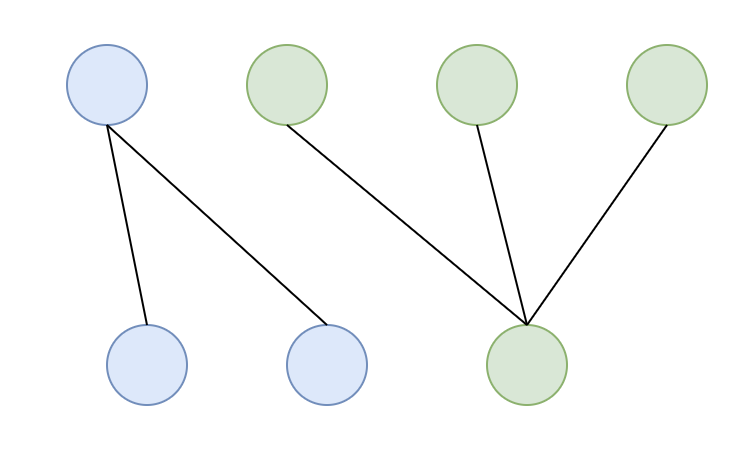
\includegraphics[scale=0.7]{matching.png}
\centering
\end{figure}

\subsection*{Repositorio}
El repositorio con todos los algoritmos se encuentran en el siguiente \href{https://github.com/Guillermo598/ProyectoADA}{link}.
\subsection*{Pregunta 1 (Voraz)}
\subsubsection*{Pseudocodigo}
Primero, presentamos un subalgoritmo que calcula los bloques de los arreglos en tiempo lineal, ya que recorre dicho arreglo una sola vez. Cabe notar que este subalgoritmo se usará en todos los algoritmos futuros. Abajo de este se encuentra el algoritmo voraz principal.
\subsubsection*{}
Recibe: un arreglo de ceros y unos

Devuelve: un arreglo de tamaños de los bloques
\begin{algorithmic}[1]
  \TITLE{\textsc{GetBlocks}$(array)$}
  \STATE $i = 1$
  \WHILE{$i < array.size$}
    \WHILE{$array[i] == 0$}
        \STATE $i = i + 1$
    \ENDWHILE
    \STATE $size = 0$
    \IF{$array[i] == 1$}
        \WHILE{$array[i] == 1$}
            \STATE $size = size + 1$
            \STATE $i = i + 1$
        \ENDWHILE
        \STATE $blocks.push(size)$
    \ENDIF
  \ENDWHILE
  \RETURN $blocks$
\end{algorithmic}
\subsubsection*{}
Recibe: dos arreglos de ceros y unos

Devuelve: un matching entre los dos arreglos y su peso
\begin{algorithmic}[1]
  \TITLE{\textsc{GreedyMinMatching}$(A, B)$}
  \STATE $blocksA = \textsc{GetBlocks$(A)$}$
  \STATE $blocksB = \textsc{GetBlocks$(B)$}$
  \STATE $m = blocksA.size$
  \STATE $n = blocksB.size$
  \IF{$m > n$} 
    \STATE $max_i = ratio = m/n$
    \STATE $j = 1$
    \FOR{$i=1$ TO m}
        \IF{$i \leq max_i$}
            \STATE $num = num + blocksA[i]$
        \ELSE
            \STATE $w = w + num/blocksB[j]$
            \STATE $num = blocksA[i]$
            \STATE $max_i = max_i + ratio$
            \STATE $j = j + 1$
        \ENDIF
        \STATE $matching.push(i,j)$
    \ENDFOR
    \STATE $w = w + num/blocksB[j]$
  \ELSE
    \STATE $max_j = ratio = n/m$
    \STATE $i = 1$
    \FOR{$j=1$ TO n}
        \IF{$j \leq max_j$}
            \STATE $den = den + blocksB[j]$
        \ELSE
            \STATE $w = w + blocksA[i]/den$
            \STATE $den = blocksB[j]$
            \STATE $max_j = max_j + ratio$
            \STATE $i = i + 1$
        \ENDIF
        \STATE $matching.push(i,j)$
    \ENDFOR
    \STATE $w = w + blocksA[i]/den$
  \ENDIF
  \RETURN $matching, w$
\end{algorithmic}

\subsubsection*{Analisis}
Dejando de lado el cálculo de los bloques de cada arreglo, el tiempo de ejecución del algoritmo propuesto es de $O(max\{m,n\})$. Esto se debe al condicional de la linea 5. Si $m$, la cantidad de bloques del arreglo $A$, es mayor, se itera asignándole un solo \textit{matching} a cada bloque de $A$. En el caso contrario, se hace lo mismo pero con los bloques de $B$. El calculo del peso del \textit{matching} $w$ se hace durante este proceso, por lo que solo le aumenta tiempo constante a la iteración. 


\subsubsection*{Implementación}
La implementación del algoritmo en C++ se puede encontrar en el siguiente \href{https://github.com/Guillermo598/ProyectoADA/blob/master/Pregunta1.cpp}{link}.
\subsection*{Pregunta 2 (Recurrencia)}
\begin{eqnarray*}
OPT(i,j) &=& 
  \begin{cases}
    A_1/sum(B_1..B_j)& \quad \text{si } i  \text{ = 1}\\
    sum(A_1..A_i)/B_1 & \quad \text{si } j \text{ = 1}\\
    OPT(i,j) = min(Agrupar(i,j), Dividir(i,j))\\
  \end{cases}
\\
Agrupar(i,j)&=&min(OPT(x,j-1)+sum(A_{x+1}..A_i)/B_j)  :\quad x\in \{1..i-1\}\\
Dividir(i,j)&=&min(OPT(i-1,y)+A_i/sum(B_{y+1}..B_j)) :\quad y\in \{1..j-1\}
\end{eqnarray*}

La siguiente imágen representa cómo funciona la recurrencia. Para calcular el OPT(6,3), mostrado de color verde, se necesita evaluar todos los de color amarillo. La subrutina Agrupar consta de la fila evaluada, mientras que Dividir evalua la columna. 
\begin{figure}[h]
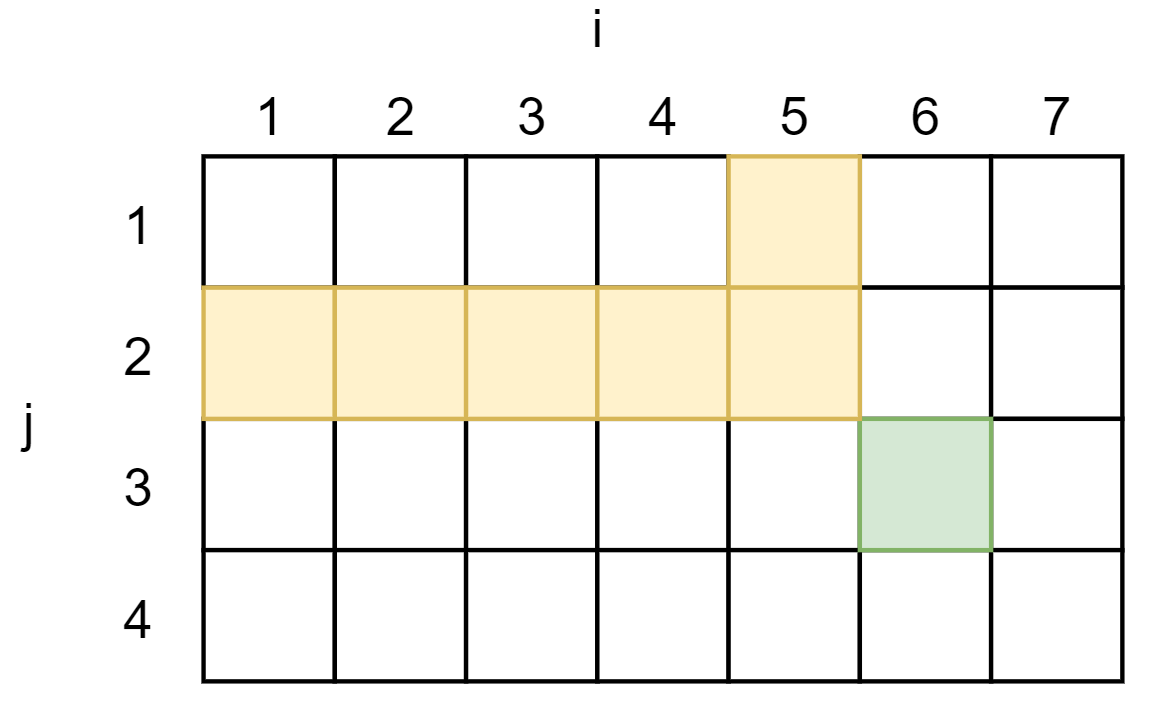
\includegraphics[scale=0.7]{tabla.png}
\centering
\end{figure}

Por ejemplo, cuando se calcula el OPT(6,3), una de las combinaciones a evaluarse es (4,2). Se calcula dicho OPT, y se le suma el peso del matching restante, como se ilustra en la figura a continuación.

\begin{figure}[h]
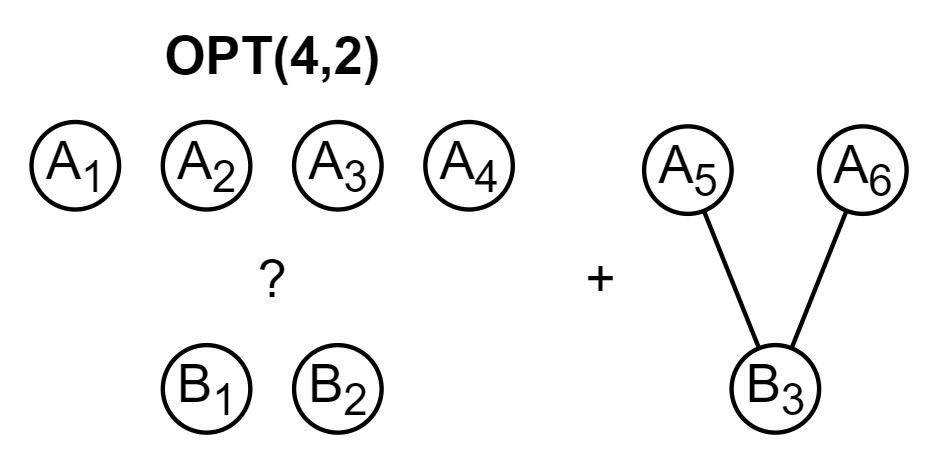
\includegraphics[scale=0.7]{ejemplo.png}
\centering
\end{figure}
\subsection*{Pregunta 3 (Recursivo)}
\subsubsection*{Pseudocódigo}
Este primer algoritmo es el principal. Transforma los arreglos a bloques y llama a la subrutina recursiva con los valores obtenidos. Esta subrutina, mostrada a continuación del primero, es la transformación de la fórmula de recurrencia presentada previamente a pseudocódigo.
\subsubsection*{}
Recibe: dos arreglos de ceros y unos

Devuelve: un matching de peso mínimo entre los dos arreglos, y el respectivo peso
\begin{algorithmic}[1]
  \TITLE{\textsc{RecursiveMinMatching}}$(A,B)$
  \STATE $blocksA = \textsc{GetBlocks$(A)$}$
  \STATE $blocksB = \textsc{GetBlocks$(B)$}$
  \STATE $m = blocksA.size$
  \STATE $n = blocksB.size$
  \RETURN $\textsc{RecursiveMinMatchingRec$(blocksA,blocksB,m,n)$}$
\end{algorithmic}
\subsubsection*{}
Recibe: dos arreglos de tamaños de bloques, y la cantidad de bloques a usar

Devuelve: un matching de peso mínimo entre los bloques usados y su peso
\begin{algorithmic}[1]
  \TITLE{\textsc{RecursiveMinMatchingRec}}$(blocksA,blocksB,i,j)$
  \IF{$i=1$}
    \STATE $w=blocksA[1]/(sum(blocksB[1]..blocksB[j])$
    \STATE $matching.push((1,1)..(1,j))$
    \RETURN $matching,w$
  \ENDIF
  \IF{$j=1$}
    \STATE $w=sum(blocksA[1]..blocksA[i])/blocksB[1]$
    \STATE $matching.push((1,1)..(i,1))$
    \RETURN $matching,w$
  \ENDIF
    \STATE $w = INF$
    \FOR{x=1 TO i-1}
        \STATE $group,w_g=\textsc{RecursiveMinMatchingRec$(blocksA, blocksB, x,j-1)$}$
        \STATE $w_g = w_g +sum(blocksA[x+1]..blocksA[i])/blocksB[j])$
        \STATE $group.push((x+1,j)..(i,j))$
        \IF{$w_g < w$}
            \STATE $w = w_g$
            \STATE $matching = group$
        \ENDIF
    \ENDFOR
    \FOR{y=1 TO j-1}
        \STATE $divide,w_d=\textsc{RecursiveMinMatchingRec$(blocksA, blocksB, i-1, y)$}$
        \STATE $w_d = w_d + blocksA[i]/sum(blocksB[y+1]..blocksB[j])$
        \STATE $divide.push((i,y+1)..(i,j))$
        \IF{$w_d < w$}
            \STATE $w = w_d$
            \STATE $matching = divide$
        \ENDIF
    \ENDFOR
    \RETURN $matching,w$
\end{algorithmic}
\subsubsection*{Análisis}
Como la llamada recursiva siempre reduce los valores de $m$ y $n$ por lo menos en 1, el árbol de recursión tendrá, a lo máximo, altura de $min(m,n)$. Además, para cualquier pares de $m$ y $n$ en los que ambos son mayores a 1, siempre llamarán dos veces al la recursión con valores $m-1$ y $n-1$, dejando de lado todas las otras llamadas. Esto quiere decir que, solo tomando una pequeña fracción de las llamadas recursivas, estas se doblan con cada nivel del arbol. Así, tenemos una cota muy inferior de $\Omega(2^{min(m,n)})$. 

Si evaluamos la recursión de forma más completa, una llamada con valores $m$ y $n$ resultan en $m+n-2$ llamadas recursivas, ya que $Agrupar$ y $Dividir$ llaman a la recursión $m-1$ y $n-1$ respectivamente. Así, podemos afirmar que la cantidad de llamadas recursivas depende más del valor máximo entre $m$ y $n$. Por lo tanto, es más preciso decir que la recursión tiene un tiempo de ejecución de $\Omega(max(m,n)^{min(m,n)})$, y eso es si el algoritmo en sí toma tiempo constante, lo cual está muy alejado de la realidad.

\subsubsection*{Implementación}
La implementación del algoritmo en C++ se puede encontrar en el siguiente \href{https://github.com/Guillermo598/ProyectoADA/blob/master/Pregunta3.cpp}{link}.
\subsection*{Pregunta 4 (Memoizado)}
\subsubsection*{Pseudocódigo}
Este primer algoritmo es el principal. Transforma los arreglos a bloques, crea los arreglos donde se guardarán los pesos con sus respectivos matching, llama a la subrutina recursiva. Esta subrutina, mostrada a continuación del primero, es el algoritmo recursivo transformado a memoizado. Los pesos y sus respectivos matching solo se cáculan si es que no han sido obtenidos previamente.
\subsubsection*{}
Recibe: dos arreglos de ceros y unos

Devuelve: un matching de peso mínimo entre los dos arreglos, y el respectivo peso
\begin{algorithmic}[1]
  \TITLE{\textsc{MemoMinMatching}}$(A,B)$
  \STATE $blocksA = \textsc{GetBlocks$(A)$}$
  \STATE $blocksB = \textsc{GetBlocks$(B)$}$
  \STATE $m = blocksA.size$
  \STATE $n = blocksB.size$
  \STATE $matching[m][n]$
  \STATE $memo[m][n] = INF$
  \RETURN $\textsc{MemoMinMatchingRec$(blocksA,blocksB,m,n,matching,memo)$}$
\end{algorithmic}
\subsubsection*{}
Recibe: dos arreglos de tamaños de bloques, la cantidad de bloques a usar, y la memoria

Devuelve: un matching entre los bloques usados de peso mínimo
\begin{algorithmic}[1]
  \TITLE{\textsc{MemoMinMatchingRec}}$(blocksA,blocksB,i,j,matching,memo)$
  \IF{$memo[i][j] \neq INF$}
    \RETURN $matching[i][j],memo[i][j]$
  \ENDIF
  \IF{$i=1$}
    \STATE $w=blocksA[1]/(sum(blocksB[1]..blocksB[j])$
    \STATE $matching[i][j].push((1,1)..(1,j))$
    \STATE $memo[i][j] = w$
    \RETURN $matching[i][j],w$
  \ENDIF
  \IF{$j=1$}
    \STATE $w=sum(blocksA[1]..blocksA[i])/blocksB[1]$
    \STATE $matching[i][j].push((1,1)..(i,1))$
    \STATE $memo[i][j] = w$
    \RETURN $matching[i][j],w$
  \ENDIF
    \STATE $w = INF$
    \FOR{x=1 TO i-1}
        \STATE $group,w_g=\textsc{MemoMinMatchingRec$(blocksA, blocksB, x,j-1,matching,memo)$}$
        \STATE $w_g = w_g +sum(blocksA[x+1]..blocksA[i])/blocksB[j])$
        \STATE $group.push((x+1,j)..(i,j))$
        \IF{$w_g < w$}
            \STATE $w = w_g$
            \STATE $matching[i][j] = group$
        \ENDIF
    \ENDFOR
    \FOR{y=1 TO j-1}
        \STATE $divide,w_d=\textsc{MemoMinMatchingRec$(blocksA, blocksB, i-1, y,matching,memo)$}$
        \STATE $w_d = w_d + blocksA[i]/sum(blocksB[y+1]..blocksB[j])$
        \STATE $divide.push((i,y+1)..(i,j))$
        \IF{$w_d < w$}
            \STATE $w = w_d$
            \STATE $matching[i][j] = divide$
        \ENDIF
    \ENDFOR
    \STATE $memo[i][j] = w$
    \RETURN $matching[i][j],w$
\end{algorithmic}
\subsubsection*{Análisis}
El tiempo de complejidad del algoritmo es $O(mn)$. Se crea una tabla $memo$ de tamaño $m*n$ para almacenar los resultados calculados por primera vez. Es decir, la recurrencia solo demora $m*n$ llamadas en llenar la tabla, y después todas las llamadas son constantes. 

\subsubsection*{Implementación}
La implementación del algoritmo en C++ se puede encontrar en el siguiente \href{https://github.com/Guillermo598/ProyectoADA/blob/master/Pregunta4.cpp}{link}.

\end{document}
